\documentclass[UTF8,14pt]{article}
\usepackage[UTF8]{ctex}
\usepackage[a4paper, margin=0.8in,top = 20mm,bottom = 20mm]{geometry}
\usepackage{fancyhdr}
\usepackage{enumerate}
\usepackage{subfigure}
\usepackage{amsmath}
\numberwithin{figure}{section}
\pagestyle{fancy}
\lhead{项目申请} % Top left header
\chead{Linux上易于裁剪的webkit浏览器} % Top center head
\rhead{谢远峰} % Top right heade
\renewcommand\headrulewidth{0.2pt} % Size of the header rule
\renewcommand\footrulewidth{0.4pt} % Size of the footer rul
\setlength{\headsep}{4mm}
\setlength{\footskip}{6mm}
\usepackage{amsmath}
\usepackage{subfigure}
\usepackage{titlesec}
\usepackage{fancyhdr} % Required for custom headers
\usepackage{lastpage} % Required to determine the last page for the footer
\usepackage{subfig,graphicx} % Required to insert images
\usepackage{enumitem}

\titleformat{\section}[hang]{\Large \bfseries}{\vspace{-1.5cm}\noindent}{0.8em}{}[\hrule]
\titleformat{\subsection}[hang]{\large \bfseries}{\quad \arabic{subsection} }{0.4em}{}[\hrule]
\titleformat{\subsubsection}[block]{\large \bfseries}{ \arabic{subsubsection} }{0.1em}{}[\hrule]

\setenumerate[1]{itemsep=0pt,partopsep=0pt,parsep=\parskip,topsep=0pt}
\setitemize[1]{itemsep=0pt,partopsep=0pt,parsep=\parskip,topsep=0pt}
\setdescription{itemsep=0pt,partopsep=0pt,parsep=\parskip,topsep=0pt}
\Huge
\title{Linux上易于裁剪的webkit浏览器}

\begin{document}
\begin{titlepage}
	\begin{center}
		\line(1,0){300}\\
		[0.65cm]
		\Huge{\bfseries 项目申请 }\\
		\line(1,0){300}\\
		\textsc{\LARGE Linux上易于裁剪的webkit浏览器}\\
		[0.5cm]
		\Large{\today}\\
		[5.5cm]
		\begin{tabular}{rl}
			申请人 :           & 谢远峰                        \\
			项目名称         : & Linux上易于裁剪的webkit浏览器 \\
			项目ID        :    & 210180685
		\end{tabular}
	\end{center}
\end{titlepage}

\section{项目简介}
目前常用开源浏览器引擎主要包括webkit,Google的blink,以及FireFox。对于嵌入式设备来说都存在体积大,功能多的问题。
基于嵌入式设备和linux系统对现有的webkit进行剪裁,将与linux无关的内核进行删除,减少内核文件的大小,使运行更行流畅
\section{项目背景}
\begin{itemize}
	\item 树莓派Linux版本\\
	      树莓派是一系列小型单板计算机。树莓派项目最初倾向于在学校和发展中国家促
	      进基础计算机科学的教学。由于其低成本、模块化和开放式设计,它被广泛应用
	      于许多领域。由于采用了 HDMI 和 USB 设备,

	      树莓派4B是流行的树莓派系列单板计算机中的最新产品,目前已经正式发布。相比
	      上一代的树莓派3B+,树莓派4B在处理器速度,多媒体性能,内存和连接方面提供了
	      突破性的增长,同时保留了向后兼容性和类似的功耗。对用户来说,树莓派4B提供的
	      桌面性能可与入门级x86 PC系统相媲美。
	\item webkit
	      \begin{figure}[ht]
		      \centering
		      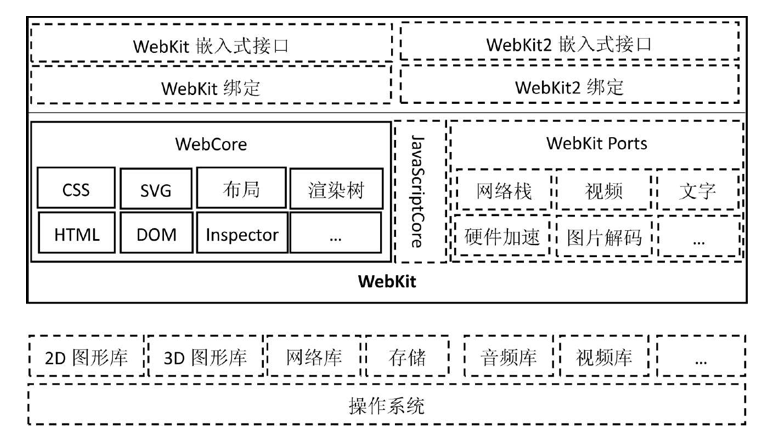
\includegraphics[width=12.00cm,height=6.78cm]{2.png}
	      \end{figure}

	      WebKit是一个开源的 Web 浏览器引擎。它是 macOS 和 iOS 中的一个框架,被许
	      多第一方和第三方应用程序使用。WebKit 代码库主要是用 C++ 编写的,包含一些 C
	      和汇编,主要是 JavaScriptCore,还有一些 Objective-C 与 Cocoa 平台集成。

	      1.底层是操作系统,WebKit 可以在不同的操作系统上工作

	      2.操作系统之上为 WebKit 依赖的第三方库,是 WebKit 运行的基础

	      3.\ WebCore 部分包含了目前被各个浏览器所使用的共享部分,是加工渲染网页的基础。

	      4.\ JavaScriptCore 引擎是 WebKit 中的默认 JavaScript 引擎。

	      5.\ WebKit Ports 指的是 WebKit 中的非共享部分,包括硬件加速架构、网络栈、视频解码、图片解码等。

	      6.\ WebCore 和 WebKit Ports 之上的层主要提供嵌入式编程接口,提供给浏览器调用。

	      7.\ WebKit2 嵌入式接口不是 WebKit 嵌入式接口的简单修改,而是为了浏览环境的安全性和稳定性原因考虑而引入了跨进程的架构。
	\item Buildroot技术\\
	      Buildroot是Linux平台上一个构建嵌入式Linux系统的框架。整个Buildroot是由Makefile脚本和Kconfig配置文件构成的。使用方法类似编译Linux内核,通过buildroot配置,menuconfig修改,编译出一个完整的可以直接烧写到机器上运行的Linux系统软件(包含boot、kernel、rootfs以及rootfs中的各种库和应用程序)。
	\item WPE\\
	      WPE直译过来是嵌入式网络平台,是使用wayland+webkit, 直接在嵌入式系统上运行webkit。
	      WPE 是嵌入式系统的官方端口,它为webkit提供的架构添加了新层,允许更容易交换的后端(图形层、窗口等)和更简单的绑定,用于基于 Linux 的系统中的编程顶层控制。
	\item 支持Kconfig\\
	      Kconfig对应内核的配置菜单。假如要想添加新的驱动到内核的源码中,可以通过修改Kconfig来增加对驱动的配置菜单,这样就有途径选择我们的驱动,假如想使这个驱动被编译,还要修改该驱动所在目录下的Makefile。
	\item Menuconfig\\
	      Linux内核的配置系统由三个部分组成,分别是:

	      1、Makefile:分布在 Linux 内核源代码根目录及各层目录中,定义 Linux 内核的编译规则;

	      2、配置文件(config.in):为用户提供配置选择的功能;

	      3、配置工具:包括配置命令解释器(对配置脚本中使用的配置命令进行解释)和配置用户界面(提供基于字符界面、基于 Ncurses 图形界面的用户配置界面,各自对应于 Make config、Make menuconfig)。

	      Linux 内核的编译菜单方法:

	      1)make config:进入命令行,逐行配置,不方便使用。

	      2)make menuconfig:图形化界面选择配置(选择方式)

	      Menuconfig界面是通过配置内核顶层的Kconfig产生的,而当输入make menuconfig命令的时候系统会读取Makefile来解析Kconfig。通常会在Kconfig里面编写以下四项:
	      模块的名字,用module开头;选项,通常设为bool(二选一)或者trastate(三选一);默认选项;帮助说明。
\end{itemize}
\section{项目需求}
\begin{enumerate}
	\item 基于树莓派4B的Linux版本,使用buildroot的方式编译完整的webkit浏览器
	\item 树莓派4B上跑的浏览器程序,以WPE方式运行,而不依赖于GTK+或Qt
	\item 几个部分变成模块化的,包括图片格式支持,JavaScriptCore,图形渲染引擎等
	\item 支持Kconfig,使用menuconfig方式配置webkit浏览器编译选项
\end{enumerate}
\section{项目方案}
\begin{enumerate}
	\item 开发流程文档完善\\
	      明确开发流程,为工作开展提供计划性指导;与项目导师进行需求沟通,明确项目需求
	\item 进行Linux版本挑选安装\\
	      基于项目需求选取对应的Linux版本,并查看内核编译配置,为后期MenuConfig的修改做准备
	\item 下载安装buildroot\\
	      从Github代码库下载对应的文件,进行下载安装和使用说明熟悉
	\item 虚拟平台上编译完整webkit
	\item 阶段总结和文档撰写
	      对于编译的完整过程进行进行溯源和详细叙述,便于后期项目复现和问题锁定时查询
	\item 基于现有webkit进行剪裁\\
	      深入了解webkit的组成结构及内容,确认待剪裁的位置,并进行阶梯式剪裁和测试
	\item 利用树莓派工具进行调试\\
	      在上述步骤成功后,将其烧写至嵌入式设备树莓派4B中
	\item 阶段总结和文档撰写\\
	      对于剪裁部分选取和过程进行详细叙述,并与项目导师进行确认
	\item 模块化部分组件\\
	      重构或编写程序将组件进行模块化
	\item 虚拟机和硬件测试\\
	      进行功能性和稳定性测试
	\item 修改内核编译配置Menuconfig\\
	      查看相关文旦,进行Menuconfig内容整理并进行修改,分别进行虚拟机和硬件测试
	\item 阶段总结和文档撰写\\
	      将模块化过程和内核编译配置进行日志记录梳理
\end{enumerate}
% \section{项目核心}
\section{计划安排}
\begin{enumerate}
	\item 07/01-07/05\\
	      开发需求确认及完善,相关基础知识梳理
	\item 07/06-07/20\\
	      进行linux、buildroot下载安装,进行webkit完整配置,并进行项目进度汇报
	\item 07/21-08/07\\
	      webkit剪裁,虚拟机编译测试
	\item 08/08-08/25\\
	      模块化组件及Menuconfig内容梳理并进行相关修改
	\item 08/26-09/20\\
	      将所有内容进行虚拟机编译,硬件测试,进行文档撰写
\end{enumerate}

\end{document}